
%!!! Calculations result and graphs here !!!%

\subsection{График зависимостей R(Q)}

Построил график для зависимостей R(Q) при разных температурах. \\График представлен на Рис. 3. \\

\begin{center}
    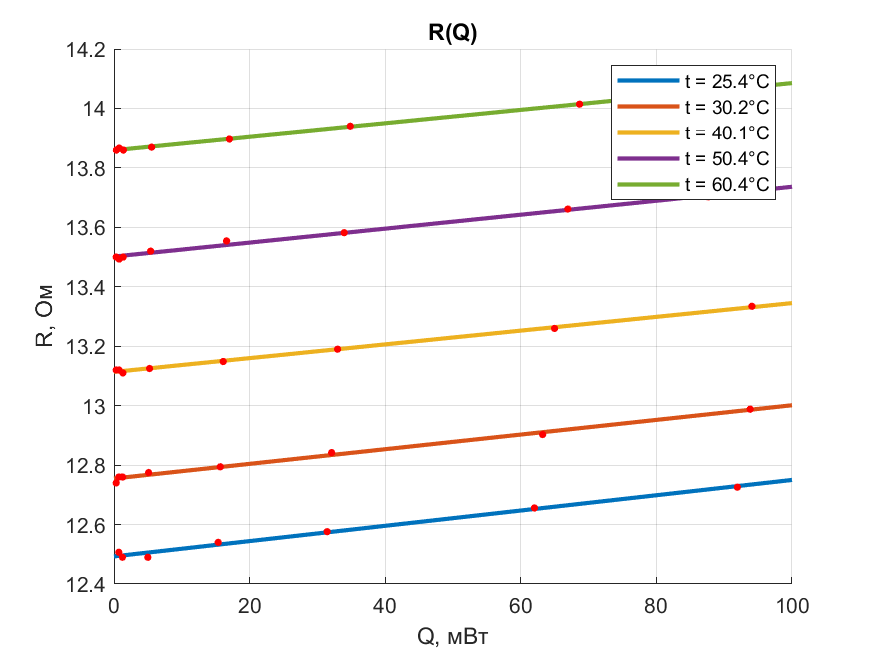
\includegraphics[scale = 1.3]{picks/223_R(Q).png} \\
    \textit{\textcolor[HTML]{000000}{Рис. 3. R(Q) для разных температур}}
\end{center}

\vspace{0.5cm}

    \begin{table}[h!]
    	\begin{center}
    		\caption*{\color[HTML]{000000}Таблица 2: Значения угловых к-тов и значения R(0) для графика R(Q)}
    		\begin{tabular}{|P{3cm}|P{1.3cm}|P{1.3cm}|P{1.3cm}|P{1.3cm}|P{1.3cm}|}
    		\hline

                \mth{t, ^\circ C}    		& 25,4  & 30,2  & 40,1  & 50,4  & 60,4 \\  
    		    \hline
    		    R(0), Ом                    & 12,49 & 12,75 & 13,11 & 13,50 & 13,86 \\
    		    \hline
                \mth{\frac{dR}{dQ}, \frac{\text{Ом}}{\text{Вт}}}  & 2,57 & 2,46 & 2,31 & 2,34 & 2,25 \\


            \hline    		
    		\end{tabular}
    	\end{center}
    \end{table}

\newpage

\subsection{График зависимости R(t)}

Построил график для зависимости R(t). \\График представлен на Рис. 4. \\

\begin{center}
    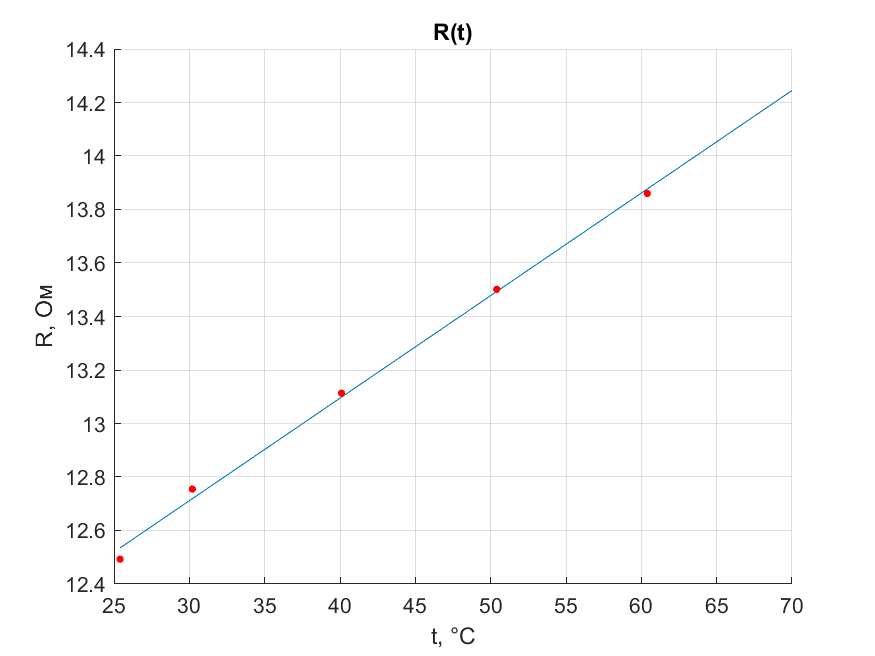
\includegraphics[scale = 1.3]{picks/223_R(T).png} \\
    \textit{\textcolor[HTML]{000000}{Рис. 4. R(t)}}
\end{center} 

\vspace{0.5cm}

Значение углового к-та для данного графика \mth{\frac{dR}{dT} = 3,83\cdot10^{-2} \frac{\text{Ом}}{K}}

\newpage

\subsection{}
